\documentclass{article}
\usepackage{graphicx} % Required for inserting images
\usepackage{amsmath, amssymb, mathtools, dirtytalk}

\graphicspath{{Images/}}

\setlength{\oddsidemargin}{0in}
\setlength{\textwidth}{6.5in}
\setlength{\topmargin}{-.55in}
\setlength{\textheight}{9in}
\pagestyle{empty}


\title{Scientific Computation II HW3}
\author{Michael Nameika}
\date{March 2023}

\begin{document}

\maketitle

\section*{Chapter 12 Problems}
\textbf{2.} Write a MATLAB program to implement (6.8) and (6.9) and construct the differentiation matrix $D_N$ associated with an arbitrary set of distinct points $x_0, \dots, x_N$. Combine it with \textbf{gauss} to create a function that computes the matrix $D_N$ associated with Legendre points in $(-1,1)$. Print results for $N = 1,2,3,4$.
\newline\newline\newline
Implementing (6.8) and (6.9) in MATLAB (see attached diffMatTest.m file), we find the following for $N=1,2,3,4$:
\begin{center}
    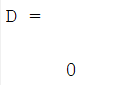
\includegraphics{GaussN=1}
    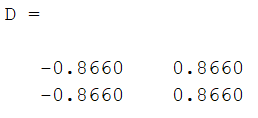
\includegraphics{GaussN=2}
    \newline\newline\newline
    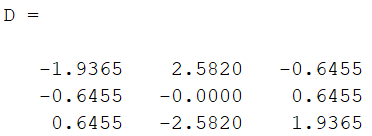
\includegraphics{GaussN=3}
    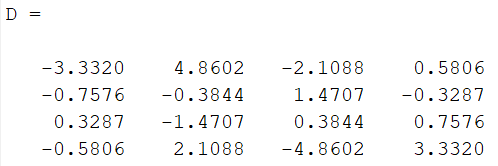
\includegraphics{GaussN=4}
    \newline\newline\newline
\end{center}
\textbf{7.} Use the FFT in $N$ points to calculate the first twenty Taylor series coefficients of $f(z) = \log(1 + \frac{1}{2}z)$. What is the asymptotic convergence factor as $N \to \infty$? Can you explain this number?
\newline\newline
Notice for a function $f(z)$, we may consider Taylor expanding on the unit circle such that 
\[f(e^{i\theta_n}) = \sum_{k = 0}^{N-1}a_ke^{i\theta_k}\]
Notice that this is the discrete Fourier transform of the Taylor coefficients. Then by using the inverse DFT, we have
\[a_n = \frac{1}{N}\sum_{k=0}^{N-1}f(\theta_k)e^{-i\theta_kn}\]
Implementing this into MATLAB (see attached fourierTaylorTest.m script), we find the following plot of the error in the first 20 coefficients:
\begin{center}
    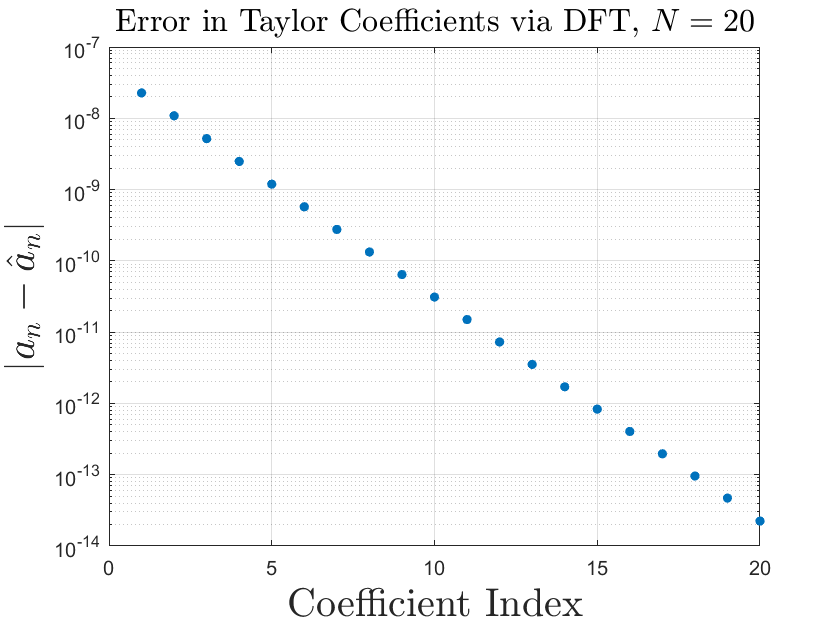
\includegraphics[scale = 0.5]{errInDFTCoeffs}
\end{center}
We also find the error in the first coefficient $a_1$ for $1 \leq N \leq 10$:
\begin{center}
    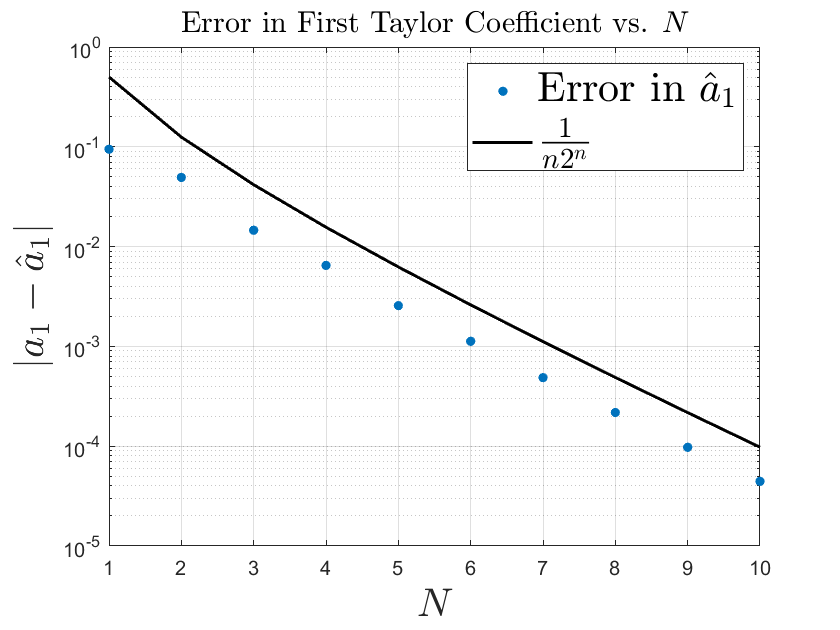
\includegraphics[scale = 0.5]{errInFirstDFTTaylorCoeff}
\end{center}
Notice that it appears the asymptotic convergence factor is roughly $\frac{1}{n2^n}$. Notice that this is the same convergence factor as the Taylor coefficients for $\log(1 + \frac{1}{2}z)$. That is, the Taylor coefficients computed via the DFT converges to the true value as $N \to \infty$ at the same rate as the Taylor coefficients converge to 0.


\section*{Chapter 13 Problems}
\textbf{3.} Modify Program 19 (p. 82) to solve $u_{tt} = u_{xx}$ as before but with initial and boundary conditions
\[u(x,0) = 0, \:\:\:\: u_x(-1,t) = 0, \:\:\:\: u(1,t) = \sin(10t)\]
Produce an attractive plot of the solution for $0 \leq t  \leq 5$.
\newline\newline\newline
Implementing this problem in MATLAB (see attached myp19.m file), we find the following solution plot for $0 \leq t \leq 5$:
\begin{center}
    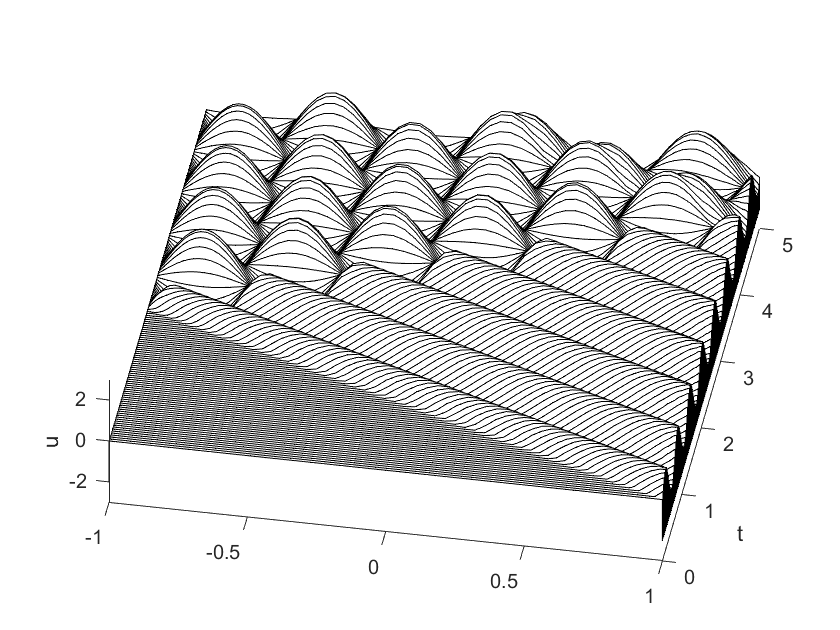
\includegraphics[scale = 0.6]{p19Plot}
\end{center}


\textbf{4.} The time step in Program 37 is specified by $\Delta t = 5/(N_x + N_y^2)$. Study this discretization theoretically and, if you like, numerically, and decide: is this the right choice? Can you derive a more precise stability limit on $\Delta t$?
\newline\newline\newline
For the stability region of the leapfrog method, we have that (along with the fourier discretization), $\Delta t < 4/N_x$. From the Chebyshev differentiation, we have that $\Delta t < \frac{9}{N_y^2}$. That is, we require that 
\[\Delta t < \min\left\{\frac{9}{N_y^2}, \frac{4}{N_x}\right\}\]
Since $\frac{4}{N_y^2 + N_x} < \min\left\{\frac{9}{N_y^2}, \frac{4}{N_x}\right\}$, a more precise stability limit would be 
\[\Delta t < \frac{4}{N_y^2 + N_x}\]
I think

\section*{Chapter 14 Problems}
\textbf{1.} Determine the first five eigenvalues of the problem
\[u_{xxxx} + u_{xxx} = \lambda u_{xx}, \:\:\:\:\: u(\pm 2) = u_x(\pm 2) = 0, \:\:\:\: -2 < x < 2,\]
and plot the corresponding eigenvectors. 
\newline\newline\newline
To begin, we must transform this problem from $-2 \leq 2$ to $-1 \leq x \leq 1$ by the transformation $t = x/2$, we have that the $nth$ order differentiation matrices must be multiplied by $1/2^n$ since $d/dt u(t) = 1/2d/dx u(x)$. Implementing this into MATLAB, we find the following figure of the first five eigenvalues and eigenvectors:
\begin{center}
    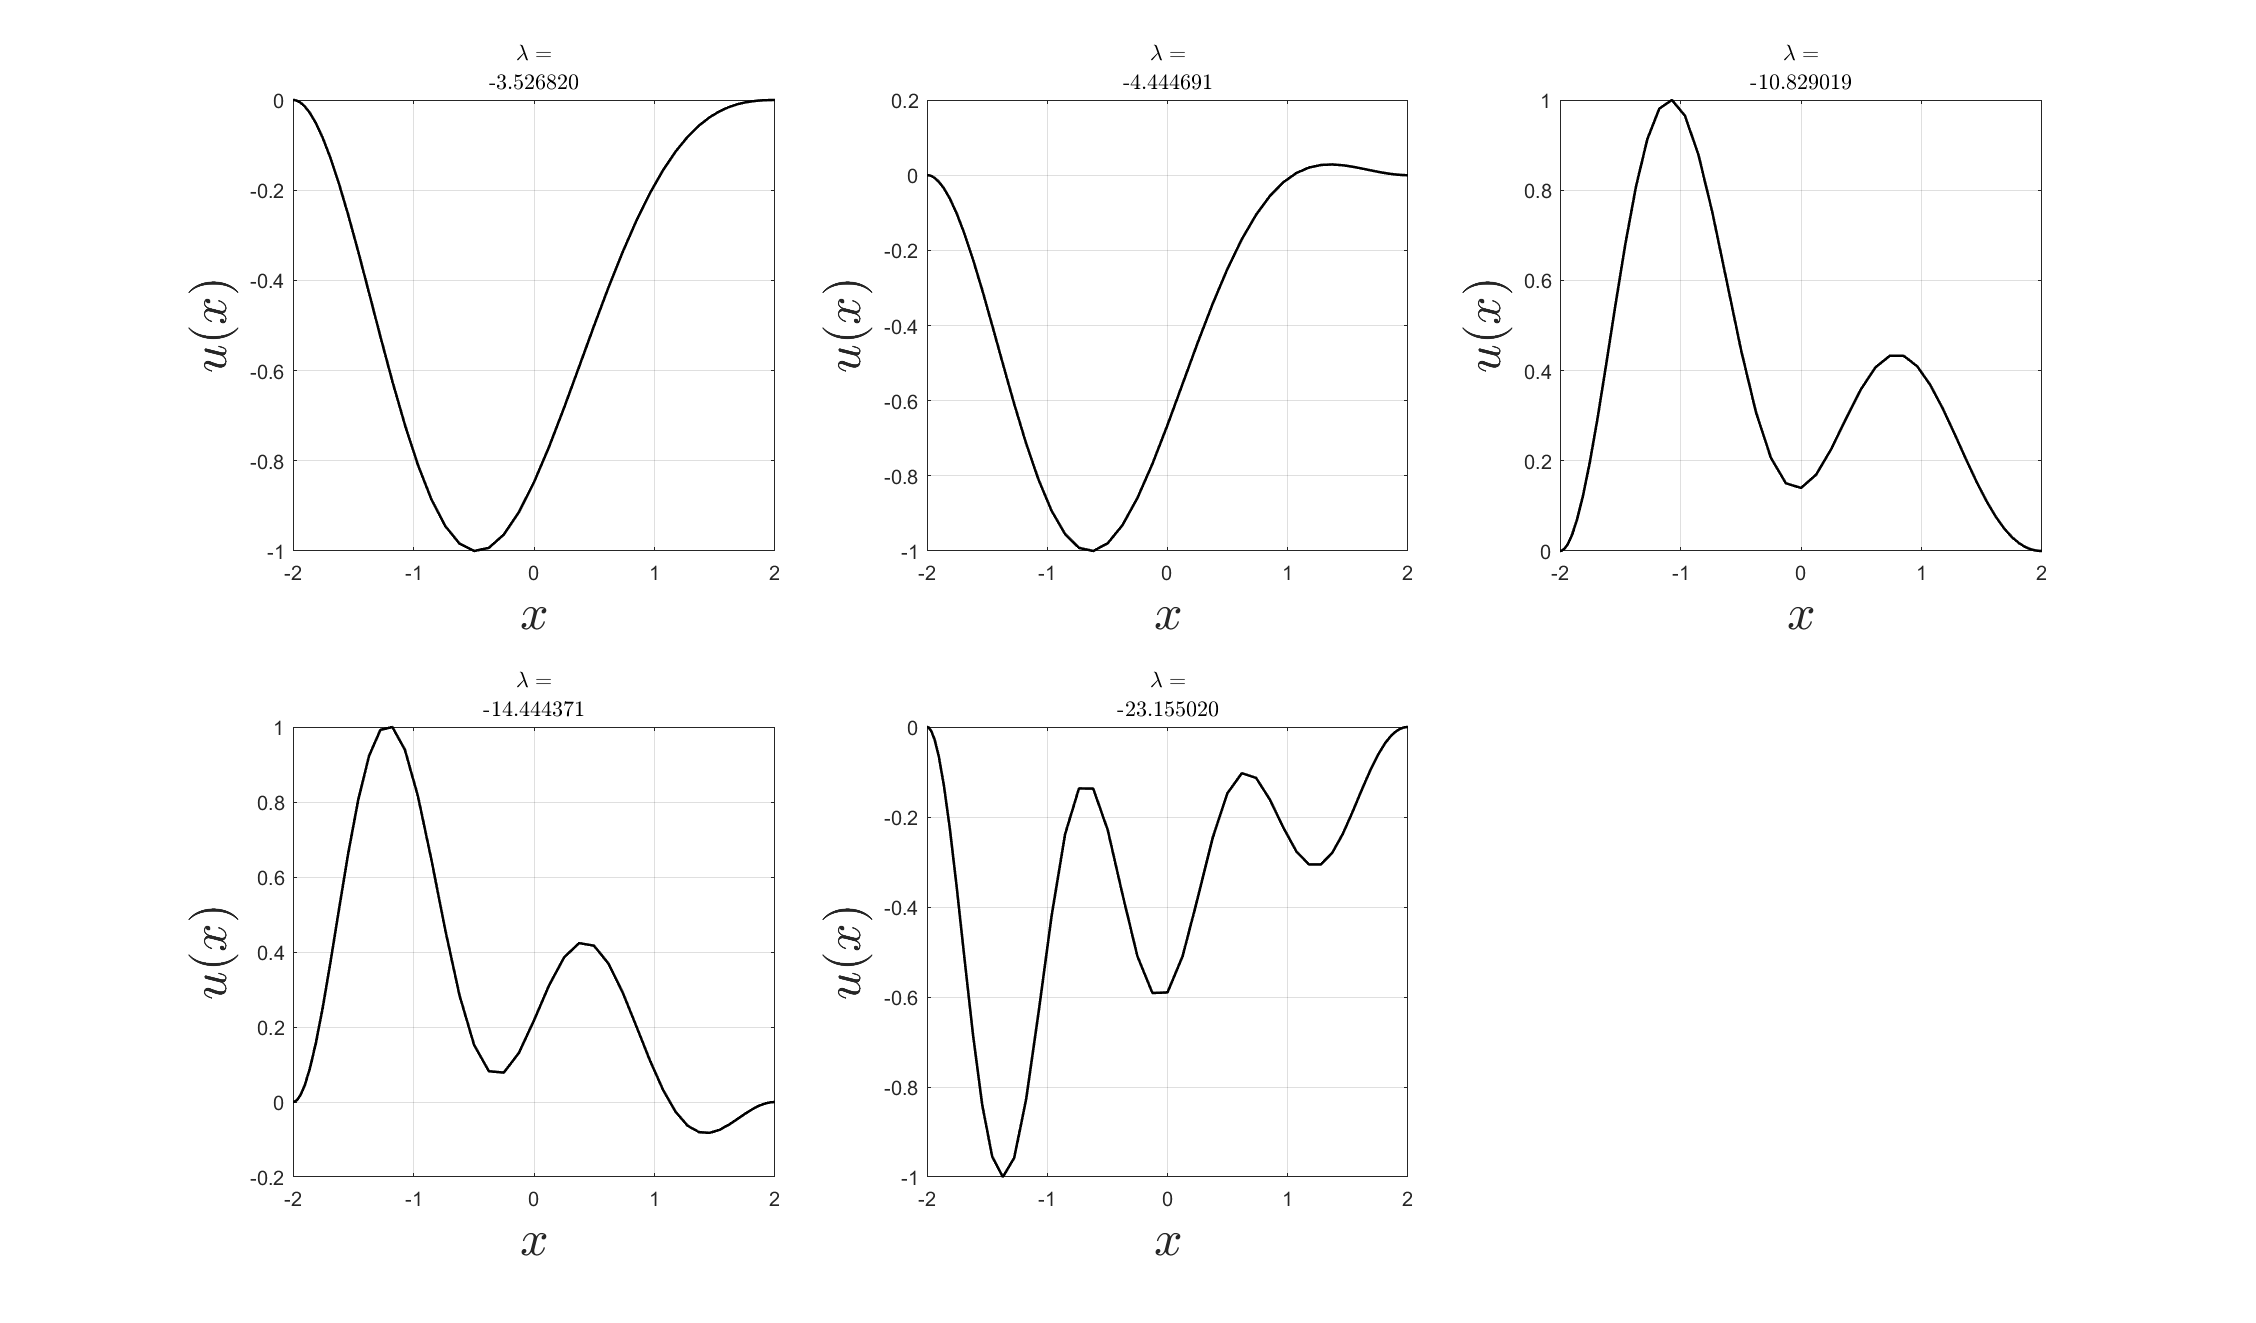
\includegraphics[scale = 0.3]{prob14_1_plot}
\end{center}


\end{document}
